\chapter{Semantische Analyse} \label{chap:semantic}

Die semantische Analyse ist notwendig, da ein syntaktisch korrektes Programm logische Fehler beinhalten kann. Ein Beispiel dafür ist in \cref{lst:semantic-error} zu sehen. Darin wird eine Variable gelesen, bevor diese definiert wurde. Ein weiterer Fehler wäre es beispielsweise eine Funktion mit zu wenigen Parametern aufzurufen. Die Aufgabe der semantischen Analyse ist es, den erzeugten \ac{ast} zu durchlaufen und dabei die einzelnen Knoten auf solche Fehler zu prüfen.

\begin{lstlisting}[language=c, caption=Inhalt der generierten BaseVisitor-Klasse, label={lst:semantic-error}]
	var r0 := r1;
	var r1 := 2;
\end{lstlisting}

\section{Abbilden auf eine Datenstruktur}
Um logische Fehler zu erkennen bietet es sich an eine eigene Datenstruktur zu entwerfen, welche das Programm abbildet und beim Durchlaufen des \ac{ast} diese Datenstruktur zu füllen. So kann, beispielsweise bei einem Funktionsaufruf, in der Datenstruktur nachgesehen werden, ob die entsprechende Funktion bereits deklariert wurde oder noch nicht. Ein weiterer Vorteil davon eine solche Datenstruktur zu definieren ist es, dass nach dem erfolgreichen Befüllen die Datenstruktur ausschließlich ein syntaktisch und semantisch korrektes Programm abbildet. Es wäre denkbar, die erzeugte Datenstruktur in einem nächsten Schritt anhand der gesammelten Daten zu optimieren und beispielsweise unbenutzte Funktionen zu entfernen, dies geschieht im aktuellen Stand der Arbeit nicht. 

In \cref{pic:Semantic-Struct} ist zu sehen, wie ein While-Programm auf eine Java-Klasse abgebildet wird. Elemente aus dem \ac{ast}, welche nicht relevant für die semantische Überprüfung oder die Codegenerierung sind, wie beispielsweise Semikolon oder Schlüsselwörter werden nicht in die Datenstruktur mit aufgenommen, sondern ausschließlich Daten wie beispielsweise Variablennamen, Werte einer Zuweisung, Name, Funktionsnamen und Anzahl von Funktionsparametern.

\begin{figure}[h!]
	%\includegraphics[width=1\textwidth]{content/pictures/LoRaWAN-OSI.JPG}
	\centering
	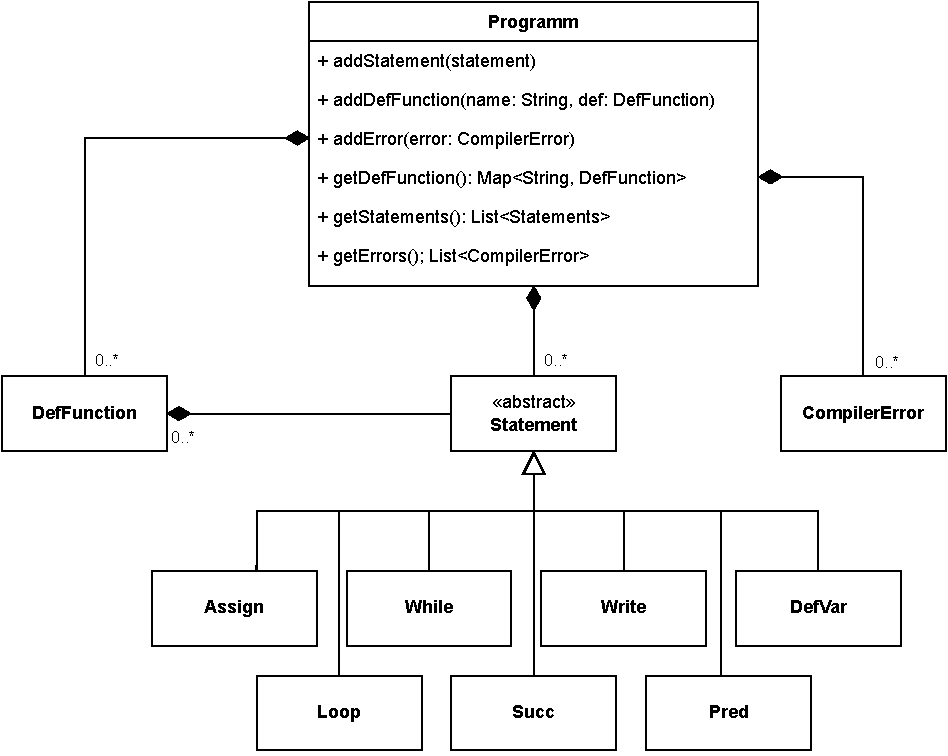
\includegraphics[width=13cm]{content/pictures/ClassDia.pdf}
	\caption{Ausschnitt der Datenstruktur}
	%	\source{\cite[S. 5]{SemtechCorporation.2020}}
	\label{pic:Semantic-Struct}
\end{figure}

\section{Durchlaufen des \acl{ast}}
\ac{antlr} erzeugt beim Visitor-Ansatz, für welchen sich bei dieser Arbeit entschieden wurde, eine \enquote{BaseVisitor}-Klasse, welche für jeden Knoten eine Visit-Methode mit einem Parameter implementiert, welcher Informationen zum entsprechenden Knoten beinhaltet. In dieser Arbeit wurde für jeden Knoten eine Visitor-Klasse erstellt, welche von dieser Baseklasse erbt und die entsprechende Visit-Methode implementiert. Mithilfe der Informationen aus dem Parameter können wiederum die Unterknoten durchlaufenen werden. Jede Visit-Methode gibt zum Schluss eine 

\begin{lstlisting}[language=java, caption=Inhalt der generierten BaseVisitor-Klasse, label={lst:parser-basevisitor}]
	public class WhileBaseVisitor<T> extends ... {
		@Override public T visitProg(ProgContext ctx) { return visitChildren(ctx); }
		@Override public T visitRead(ReadContext ctx) { return visitChildren(ctx); }
		...
	}
\end{lstlisting}